\section{Password Similarity}
\begin{center}
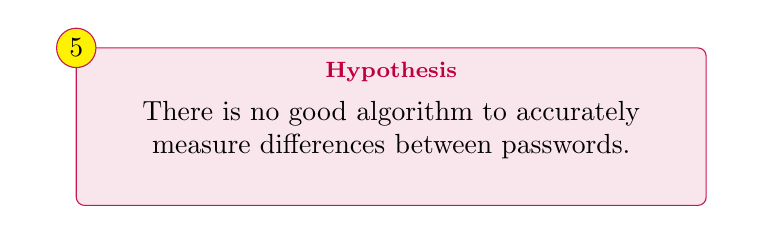
\begin{tikzpicture}
    \def\gridwidth{8}
    \def\gridheight{2}

    % Draw the main grid
    \draw[fill=purple!10, draw=purple!90, rounded corners=3pt,] (0,0) rectangle (\gridwidth,\gridheight);

    \node[align=center, text=purple, font=\footnotesize] (box1) at (\gridwidth/2,\gridheight-0.3) {\bf Hypothesis};
        
    \node[below, text width=9cm, align=center] at (box1.south) {There is no good algorithm to accurately measure differences between passwords.};
    
    \node[circle,fill=yellow,inner sep=0pt,minimum size=0.5cm, draw=purple!90] at (0,\gridheight) {5};
\end{tikzpicture}
\end{center}

The problem of password similarity is closely related to string matching. Though, measuring password similarity is more difficult than normal strings. The text transformations (such as reversals), phonetic changes, and concatenation of other words and symbols increase the difficulty.

Password similarity algorithms are important and have many use-cases. In password strength meters, we want to understand how close is the user password to existing passwords that we might deem weak. If we are developing an algorithm to generate passwords, then we might need an algorithm to measure the difference between the generated and the true password. A password similarity algorithm assumes we have a model of the password.

The classical methods such as edit distance (e.g. Levenshtein distance) are not great approximates for passwords. The transformations in passwords can greatly skew the similarity metric.

In \cite{das_tangled_2014}, Das. et al. discuss various similarity algorithms:

\begin{itemize}
    \item Distance-like. Manhattan, Cosine, etc.
    \item Edit-distance. Levenshtein, Damerau-Levenshtein functions.
    \item Token-based distance. Dice, Overlap.
    \item Alignment-like. Smith-Waterman, Neddleman Wunsch, LCS.
    \item Embedding:
        \begin{itemize}
            \item pass2path \cite{pal_beyond_2019} (Pal et al.). Uses FastText.
            \item CWAE \cite{pasquini_improving_2021} (Pasquini et al.)
            \item Other Neural Embedding (Word2Vec, GloVe, FastText, ELMo, BERT, etc.)
        \end{itemize}
\end{itemize}


\begin{itemize}
\item Distance-like
    \begin{itemize}
    \item Manhattan
    \item Cosine
    \end{itemize}
    
\item Edit-distance
\begin{itemize}
    \item Levenshtein
    \item Damerau-Levenshtein
    \item Jaro-Winkler
\end{itemize}

\item Token-based distance
\begin{itemize}
    \item Dice
    \item Overlap
\end{itemize}

\item Alignment-like
\begin{itemize}
    \item Smith-Waterman
    \item Needleman-Wunsch
    \item Longest Common Subsequence (LCS)
\end{itemize}

\item Phonetic encoding
\begin{itemize}
    \item Soundex
    \item Metaphone
\end{itemize}

\item N-gram based similarity

\item Keyboard distance metrics
\begin{itemize}
    \item Keyboard Coordinate Representation
    \item Keyboard Key Press Metric
\end{itemize}

\item Markov Chain models

\item Embedding
\begin{itemize}
    \item pass2path \cite{pal\_beyond\_2019} (Pal et al.)
    \item CWAE \cite{pasquini\_improving\_2021} (Pasquini et al.)
    \item FastText embeddings
    \item Siamese networks
\end{itemize}

\item Structural similarity
\begin{itemize}
    \item Essential Transformation Sequence (ETS)
\end{itemize}

\end{itemize}

\noindent\begin{tikzpicture}
\node[draw,rectangle,rounded corners=2pt,inner sep=10pt,outer sep=0pt] (box) {
\begin{minipage}{\columnwidth - 20pt}
\footnotesize
\centering

\textbf{Example of transformations}

\newline

\texttt{321drowssap} $\rightarrow$ \texttt{password123}

\end{minipage}
};
\end{tikzpicture}

We need to define what a similar password means. Then compare the various algorithms based on some criteria, such as complexity in time, space, accuracy, and etc.

\begin{table}[h]
\centering
\footnotesize
\caption{Time and Space Complexity of Password/String Similarity Algorithms}
\begin{tabular}{lcc}
\textbf{Algorithm} & \textbf{Time} & \textbf{Space} \\
\midrule
\multicolumn{3}{c}{\textbf{Distance-like}} \\ \hline
Manhattan & O(n) & O(1) \\
Cosine & O(n) & O(1) \\
\multicolumn{3}{c}{\textbf{Edit-distance}} \\ \hline
Levenshtein & O(mn) & O(mn) \\
Damerau-Levenshtein & O(mn) & O(mn) \\
\multicolumn{3}{c}{\textbf{Token-based distance}} \\ \hline
Dice & O(n+m) & O(n+m) \\
Overlap & O(n+m) & O(n+m) \\
\multicolumn{3}{c}{\textbf{Alignment-like}} \\ \hline
Smith-Waterman & O(mn) & O(mn) \\
Needleman-Wunsch & O(mn) & O(mn) \\
LCS & O(mn) & O(mn) \\
\multicolumn{3}{c}{\textbf{Embedding}} \\ \hline
Neural Embedding & O(n) (training) & O(n) \\
Neural Embedding & O(n) (inference) & O(n) \\
\bottomrule
\end{tabular}
\end{table}

\begin{enumerate}
\item Word2Vec (Word-level):
\begin{itemize}
\item Technique: Word2Vec uses a shallow neural network to learn word embeddings. It comes in two flavors: Continuous Bag-of-Words (CBOW) and Skip-gram. CBOW predicts a target word given its context, while Skip-gram predicts the context words given a target word.
\item Difference: Word2Vec is a straightforward and computationally efficient model that captures semantic and syntactic relationships between words.
\end{itemize}


Copy code
\item GloVe (Word-level):
\begin{itemize}
    \item Technique: GloVe (Global Vectors) learns word embeddings by factorizing a matrix of word co-occurrence statistics. It combines global matrix factorization and local context window methods.
    \item Difference: GloVe takes into account global word-word co-occurrence statistics, which can capture more global relationships compared to Word2Vec.
\end{itemize}

\item FastText (Word-level and Character-level):
\begin{itemize}
    \item Technique: FastText is an extension of Word2Vec that includes character-level information. It represents each word as a bag of character n-grams, allowing it to capture subword information and handle out-of-vocabulary words.
    \item Difference: FastText can generate embeddings for unknown words based on their character n-grams, making it useful for morphologically rich languages and handling rare or misspelled words.
\end{itemize}

\item ELMo (Character-level):
\begin{itemize}
    \item Technique: ELMo (Embeddings from Language Models) generates word embeddings using a bidirectional LSTM trained on a large text corpus. It captures context-dependent word representations by considering the entire sentence.
    \item Difference: ELMo provides dynamic word embeddings that change based on the context in which the word appears, allowing it to capture polysemy and contextual information.
\end{itemize}

\item BERT (Subword-level):
\begin{itemize}
    \item Technique: BERT (Bidirectional Encoder Representations from Transformers) uses a transformer architecture to learn contextual word representations. It is trained on a masked language modeling task and a next sentence prediction task.
    \item Difference: BERT captures bidirectional context and can generate different representations for the same word based on its surrounding context. It uses subword tokenization to handle out-of-vocabulary words.
\end{itemize}

\item GPT (Subword-level):
\begin{itemize}
    \item Technique: GPT (Generative Pre-trained Transformer) is a language model that uses a transformer decoder architecture. It is trained on a large corpus of text to predict the next word in a sequence.
    \item Difference: GPT is a unidirectional model that generates embeddings based on the previous context. It can be fine-tuned for various downstream tasks such as text generation and classification.
\end{itemize}

\item CharacterBERT (Character-level):
\begin{itemize}
    \item Technique: CharacterBERT is a variant of BERT that operates directly on character-level input. It uses a character-level CNN and a transformer encoder to learn character-level embeddings.
    \item Difference: CharacterBERT can handle out-of-vocabulary words and capture subword information without explicit tokenization. It is particularly useful for languages with complex morphology.
\end{itemize}

\item Flair (Character-level):
\begin{itemize}
    \item Technique: Flair embeddings are generated using a character-level language model trained on a large corpus. They capture contextual information and can be combined with other types of embeddings.
    \item Difference: Flair embeddings are contextual and can be used to represent words, sentences, or documents. They have shown strong performance on named entity recognition and text classification tasks.
\end{itemize}
\end{enumerate}

\begin{enumerate}
\setcounter{enumi}{8}
\item RoBERTa (Subword-level):
\begin{itemize}
\item Technique: RoBERTa (Robustly Optimized BERT Pretraining Approach) is an optimized version of BERT. It uses dynamic masking, larger batch sizes, and more training data to improve performance.
\item Difference: RoBERTa removes the next sentence prediction task and uses only the masked language modeling objective. It also trains on longer sequences and achieves better performance than BERT on various tasks.
\end{itemize}


Copy code
\item XLNet (Subword-level):
\begin{itemize}
    \item Technique: XLNet is an autoregressive language model that uses a permutation language modeling objective. It captures bidirectional context by maximizing the expected likelihood over all permutations of the factorization order.
    \item Difference: XLNet combines the advantages of autoregressive models like GPT and autoencoding models like BERT. It can handle dependencies between masked positions and achieves state-of-the-art performance on several benchmarks.
\end{itemize}

\item ALBERT (Subword-level):
\begin{itemize}
    \item Technique: ALBERT (A Lite BERT) is a lightweight variant of BERT that uses parameter-reduction techniques. It employs factorized embedding parameterization, cross-layer parameter sharing, and a sentence ordering prediction task.
    \item Difference: ALBERT significantly reduces the number of parameters compared to BERT while maintaining comparable performance. It is designed to be more memory-efficient and faster to train.
\end{itemize}

\item ELECTRA (Subword-level):
\begin{itemize}
    \item Technique: ELECTRA (Efficiently Learning an Encoder that Classifies Token Replacements Accurately) is a transformer-based model that uses a replaced token detection objective. It trains a discriminator to predict whether each token in the input is original or replaced by a generator.
    \item Difference: ELECTRA is computationally efficient and achieves strong performance on various natural language processing tasks. It is particularly effective for tasks that require fine-grained linguistic knowledge.
\end{itemize}

\item Longformer (Subword-level):
\begin{itemize}
    \item Technique: Longformer is a transformer-based model designed to handle long sequences. It uses a combination of a local self-attention mechanism and a global attention mechanism to process long documents efficiently.
    \item Difference: Longformer can handle sequences of up to 4,096 tokens, making it suitable for tasks that require processing long-range dependencies, such as document classification and question answering.
\end{itemize}

\item ConveRT (Subword-level):
\begin{itemize}
    \item Technique: ConveRT (Conversational Representations from Transformers) is a lightweight conversational reparameterization of BERT. It uses a dual-encoder architecture and a contrastive loss function to learn representations for conversational tasks.
    \item Difference: ConveRT is specifically designed for conversational AI and achieves strong performance on tasks such as response selection and intent classification while being computationally efficient.
\end{itemize}
\end{enumerate}

\subsection{Related Work}


